\section{Direct orbit transfer analysis}

This section presents the results computed for a direct orbit transfer between
Earth and the two interstellar objects. The analysis is performed by solving the
Lambert's problem under the Keplerian assumption.

The algorithm used is the one presented by \cite{izzo2015}, as it is proven to
be more accurate and faster than other classical algorithms. The ephemerides for
'Omuaumua and Borisov are obtained from JPL Horizons API service at epoch
January 1, 2018. These have been propagated under the two-body assumption to
simplify the analysis.


\newpage
\begin{figure}[H]
  \centering
  \includegraphics[width=\textwidth]{static/oumuamua/direct-transfer-porkchop.png}
  \caption{Launch energy porkchop plot for 1I/'Oumuamua.}
  \label{fig:oumuamua-direct-transfer-porkchop}
\end{figure}
\begin{figure}[H]
  \centering
  \includegraphics[width=\textwidth]{static/borisov/direct-transfer-porkchop.png}
  \caption{Launch energy porkchop plot for 2I/Borisov.}
  \label{fig:oumuamua-direct-transfer-porkchop}
  \label{fig:borisov-direct-transfer-porkchop}
\end{figure}
